\documentclass[border=10pt]{standalone}

\usepackage{tikz}
\usepackage{tikzsymbols}
\usetikzlibrary{calc,patterns,shapes.geometric}

\def\centerarc[#1](#2)(#3:#4:#5){\draw[#1] ($(#2)+({#5*cos(#3)},{#5*sin(#3)})$) arc (#3:#4:#5);}

\begin{document}
	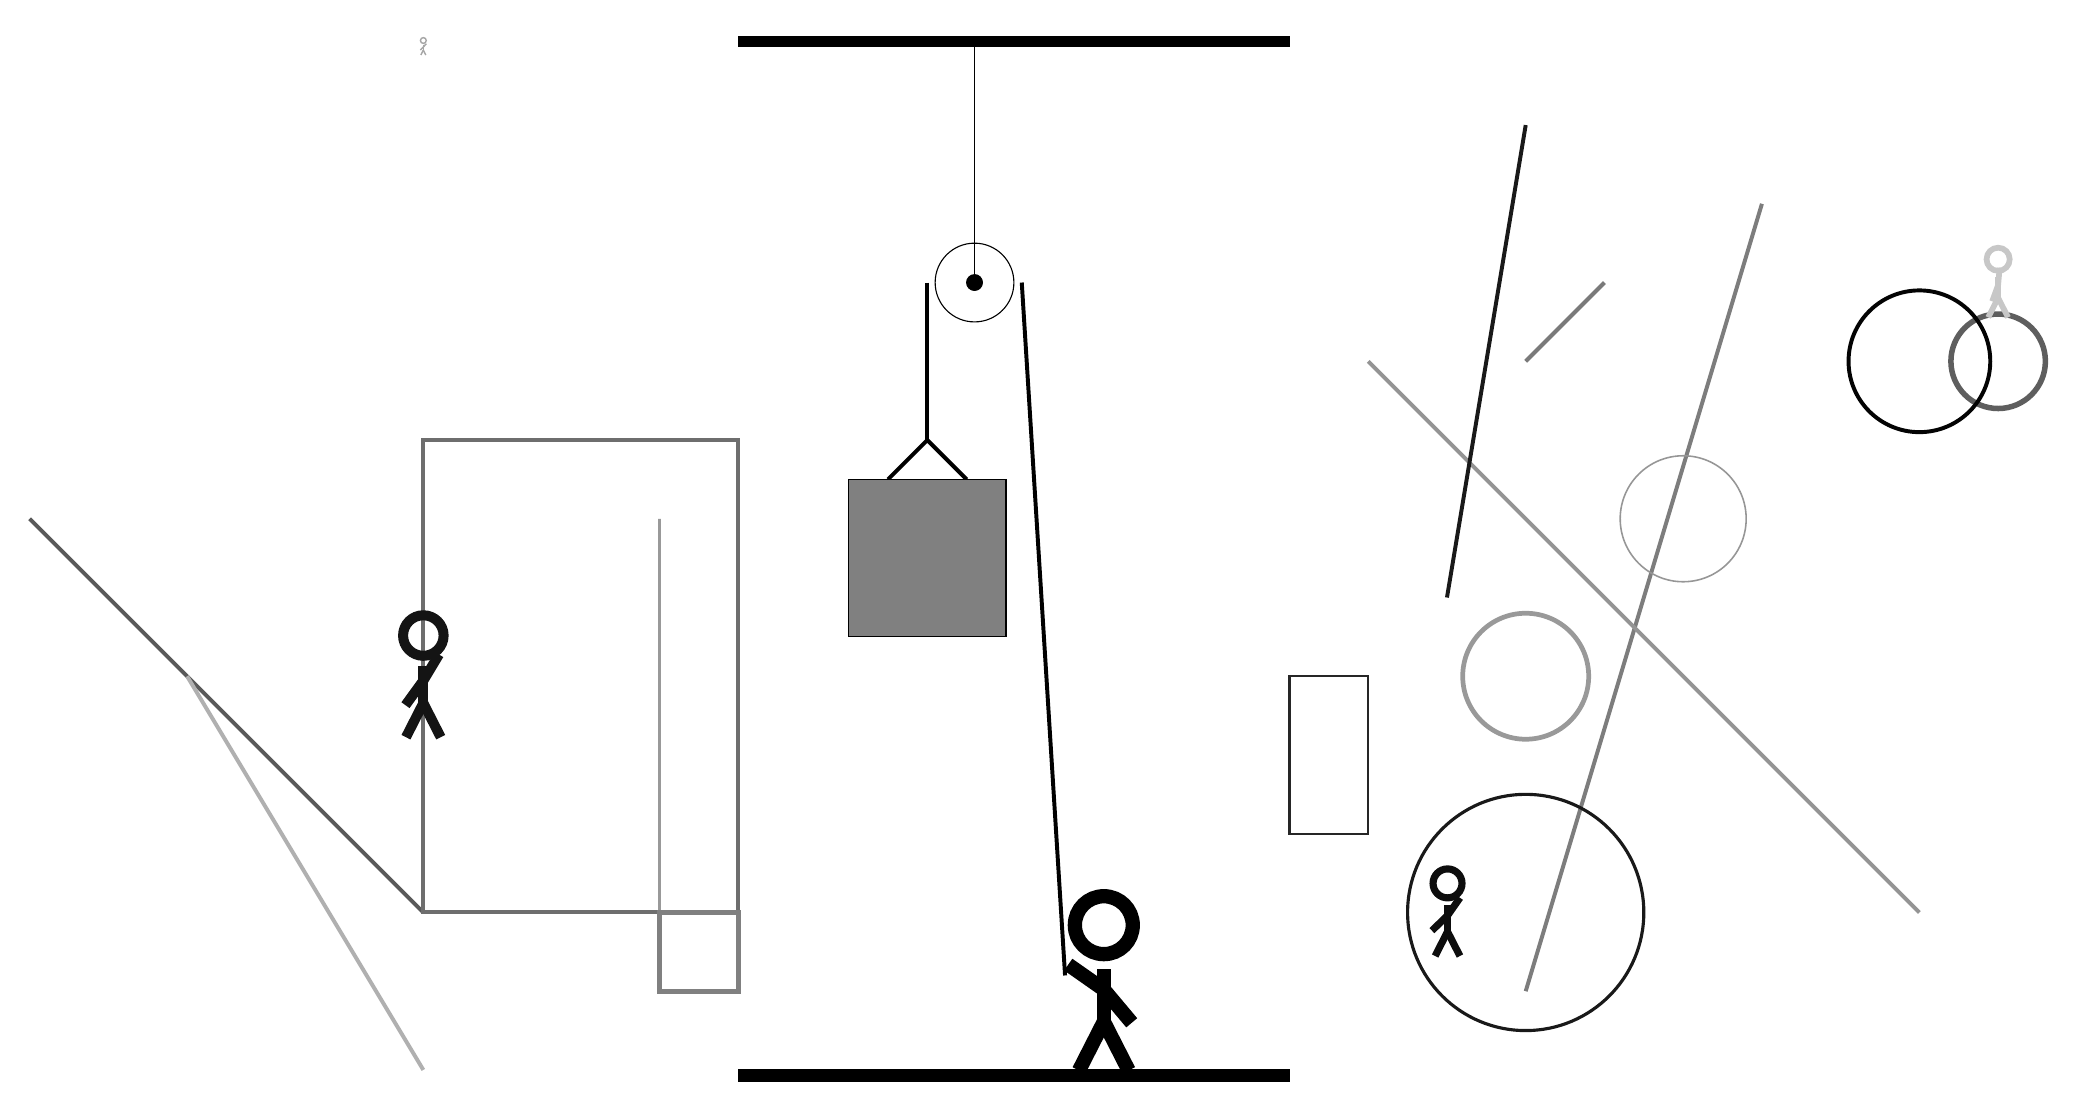
\begin{tikzpicture}
		%%%%% START %%%%%
		
		\draw[fill=black] (-2, 10) rectangle (5, 10.125);
		
		\draw (1, 7) circle (0.5);
		\draw[fill=black] (1, 7) circle (0.1);
		\draw (1, 10) -- (1, 7);
		
		\draw[line width=0.5mm] (-0.1, 4.5) -- (0.4, 5.0) -- (0.9, 4.5);
		\draw[fill=black!50] (-0.6, 4.5) rectangle (1.4, 2.5);
		
		\draw [line width=0.4mm, color=black!69](10, -2) circle (0.0);
		
		\draw [line width=0.7mm, color=black!63](14, 6) circle (0.6);
		\node[line width=0.5mm, color=black!95] at (7, -1) {\Strichmaxerl[5][44][55]};
		\draw [line width=0.6mm, color=black!40](8, 2) circle (0.8);
		\draw [line width=0.5mm, color=black!99](13, 6) circle (0.9);
		
		\draw[line width=0.5mm, color=black!65](-6, -1) -- (-11, 4);
		\draw[line width=0.3mm, color=black!85] (6, 2) rectangle (5, 0);
		
		\draw[line width=0.5mm, color=black!57] (-2, 5) rectangle (-6, -1);
		\draw[line width=0.5mm, color=black!51](8, -2) -- (11, 8);
		\draw[line width=0.4mm, color=black!40] (-3, -2) rectangle (-3, 4);
		
		\draw[line width=0.5mm, color=black!31](-6, -3) -- (-9, 2);
		
		\draw[line width=0.6mm, color=black!50] (-3, -2) rectangle (-2, -1);
		\node[line width=0.3mm, color=black!92] at (-6, 2) {\Strichmaxerl[7][54][59]};
		
		\draw [line width=0.4mm, color=black!90](8, -1) circle (1.5);
		\draw[line width=0.5mm, color=black!52](8, 6) -- (9, 7);
		\draw[line width=0.5mm, color=black!42](6, 6) -- (13, -1);
		
		\node[line width=0.5mm, color=black!22] at (14, 7) {\Strichmaxerl[4][70][85]};
		\draw[line width=0.5mm, color=black!90](8, 9) -- (7, 3);
		\node[line width=0.2mm, color=black!35] at (-6, 10) {\Strichmaxerl[1][46][46]};
		\draw [line width=0.2mm, color=black!41](10, 4) circle (0.8);
		
		\draw[line width=0.5mm] (0.4, 7) -- (0.4, 5.0);
		\centerarc[line width=0.5mm](1, 7)(0:180:0.6);
		\draw[line width=0.5mm](1.6, 7) -- (2.15, -1.8);
		
		\node at (2.6, -1.9) {\Strichmaxerl[10][-35][-50]};
		
		\draw[fill=black] (-2, -3) rectangle (5, -3.15);
		
		%%%%% END %%%%%
	\end{tikzpicture}
\end{document}